\documentclass[10pt,twocolumn,a4paper]{article}
\usepackage[margin=0.72in,top=0.78in,bottom=0.75in,columnsep=0.25in]{geometry}
\usepackage[T1]{fontenc}
\usepackage[utf8]{inputenc}
\usepackage{mathptmx}
\usepackage{courier}
\usepackage{balance}
\usepackage{placeins}
\usepackage{amsmath}
\usepackage{microtype}
\usepackage{booktabs,array,tabularx}
\usepackage{graphicx}
\usepackage{tikz}
\usetikzlibrary{arrows.meta,positioning}
\usepackage[font=small,labelfont=bf,labelsep=period]{caption}
\usepackage{titlesec}
\usepackage{fancyhdr}
\usepackage[hidelinks]{hyperref}
\hypersetup{pdftitle={From Agent Instructions to Executable Procedures: The PACT Architecture},pdfauthor={Noah Dylan Pelegrini},pdfsubject={Procedural Agent Composition and Traceability}}
\urlstyle{same}
\titleformat{\section}{\normalsize\bfseries\raggedright\hyphenpenalty=10000}{\thesection}{0.6em}{}
\titleformat{\subsection}{\normalsize\bfseries\raggedright\hyphenpenalty=10000}{\thesubsection}{0.6em}{}
\titlespacing*{\section}{0pt}{2.2ex plus .3ex minus .2ex}{1.1ex plus .2ex}
\titlespacing*{\subsection}{0pt}{1.8ex plus .2ex minus .2ex}{.8ex plus .1ex}
\setlength{\parindent}{1em}
\setlength{\parskip}{0pt}
\setlength{\headheight}{12pt}
\setlength{\textfloatsep}{12pt plus 2pt minus 2pt}
\setlength{\dbltextfloatsep}{12pt plus 2pt minus 2pt}
\setlength{\floatsep}{10pt plus 2pt minus 2pt}
\renewcommand{\topfraction}{.9}
\renewcommand{\dbltopfraction}{.9}
\renewcommand{\textfraction}{.07}
\renewcommand{\floatpagefraction}{.8}
\setcounter{topnumber}{3}
\setcounter{dbltopnumber}{3}
\pagestyle{fancy}
\fancyhf{}
\fancyhead[L]{\footnotesize PACT: Procedural Agent Composition and Traceability}
\fancyhead[R]{\footnotesize N. D. Pelegrini}
\fancyfoot[C]{\footnotesize\thepage}
\renewcommand{\headrulewidth}{0.3pt}
\raggedbottom
\emergencystretch=1em
\begin{document}
\twocolumn[{
\centering
{\LARGE\bfseries From Agent Instructions to Executable Procedures:\\[3pt] The PACT Architecture\par}
\vspace{10pt}
{\large Noah Dylan Pelegrini\par}
\vspace{3pt}
Independent Researcher\\
\href{mailto:contact@11adyy.dev}{contact@11adyy.dev}\\
\url{https://github.com/11adyy/pact-research}
\vspace{12pt}
\begin{minipage}{0.94\textwidth}
\small
\noindent\textbf{Abstract.} An agent can produce a plausible answer while leaving the procedure that produced it difficult to reuse, inspect, or constrain. This problem becomes especially apparent when a language model is asked to supply the task logic, choose tools, carry intermediate information, and decide the next action within the same interaction. We develop PACT (Procedural Agent Composition and Traceability), an architectural account of agent behavior in which procedures are explicit artifacts. A procedure, called a skill, assembles semantic operations called capabilities; named state carries information between them; and bindings select executable implementations independently of the procedure definition. The central idea is to preserve the organization of a task while allowing its computational mechanisms to change. We first establish this composition model and the boundaries of useful decomposition, then describe the runtime responsibilities needed to make it executable. A reference system realizes these responsibilities through declarative specifications, dependency scheduling, controlled state expressions, service resolution, and execution policies. We examine how the same boundaries support validation and operational accountability. Reported experiments compare single-call prompting with structured execution on decision and text-processing tasks. Structured execution exposes reusable steps and intermediate artifacts, but takes roughly 2.5 to 2.7 times as long in the evaluated configurations and exhibits slightly greater output variation. We extend this account with 23,382 controlled runtime executions: all 1,200 healthy PACT runs match exact task oracles, compatible solver substitution succeeds in 40 of 40 pairs, and native execution adds roughly 11.4--11.6 ms over a manually guarded local pipeline. Fault probes confirm specified policy blocks while exposing null and output-type validation gaps, missing-target-tenant acceptance, and effects after timeout. The combined evidence supports bounded procedural and systems claims; additional author-reported LLM aggregates remain unverified.
\end{minipage}
\vspace{16pt}
}]
\thispagestyle{plain}

\section{Introduction: Giving Agent Behavior a Procedural Form}

A useful agent often performs the same kind of work in many contexts. It may gather alternatives, assess them against stated criteria, select a course of action, and return a result. The inputs change, but much of the organization remains recognizable. Nevertheless, a common way to implement this behavior is to describe the entire job in a prompt and ask a language model to reconstruct a suitable process on each invocation. What persists is the instruction text; the procedure itself remains largely an event inside a model interaction.


This distinction matters when an agent becomes part of an operating system rather than a demonstration. Developers need to know which result was consumed by a later step, whether a tool can be replaced, where a policy must be checked, and which part of an execution should be investigated after an unexpected outcome. A final answer, even accompanied by a textual explanation, does not by itself answer these questions. They concern the organization of computation and the interfaces between its parts.


We approach the problem through a familiar property of engineered procedures: a process can encode reusable knowledge without requiring every participant to derive its organization anew. In an industrial setting, an experienced operator brings substantial judgment to a task, but that judgment operates within procedures that capture established sequencing, dependencies, and constraints. The procedure does not substitute for expertise. It gives expertise a form in which it can be applied consistently and reviewed.


PACT applies this distinction to language-model agents. Its premise is that the organization of a task should be available as an artifact that the system can execute and inspect. Such an artifact need not prescribe the internal computation of every operation. A step may still rely on a probabilistic model, an external service, or a deterministic function. What becomes explicit is the operation requested, its interface, the information it consumes, and its place in the surrounding process.


The proposal therefore begins with composition rather than with a particular execution engine. Capabilities describe meaningful operations over information. Skills organize those operations into procedures. Bindings connect the operations to available implementations. Execution state records the values that move through the procedure. Together, these elements create a boundary between a task's semantic organization and the mechanisms used to realize it.


This boundary leaves substantial work to the agent. The agent still interprets goals, decides which procedure is relevant, chooses applicable policies, handles failures at the appropriate level, and adapts its strategy to unfamiliar situations. PACT supplies an execution substrate for the procedures it selects or constructs. Known skills can be invoked directly; new tasks can be addressed through new compositions of existing capabilities.


Three questions guide the paper. First, what representation makes a procedure reusable without tying it to a specific model or tool? Second, what must a runtime do to preserve that representation during execution? Third, what operational properties and costs follow from making these boundaries explicit? We answer them in that order. The composition model and its design limits precede the reference architecture; governance and comparison then follow from the execution model; an evaluation concludes the technical account.


PACT is the revised terminology used throughout this manuscript. We retain the original benchmark observations and extend the empirical account with a separately recorded systems evaluation of the unchanged reference runtime. The extended study uses matched deterministic workloads to test execution, policy behavior, substitution, and cost; reported LLM aggregates are identified separately according to their evidence status.


\section{The Composition Model}

\subsection{A Skill Is a Procedure, Not a Prompt Container}

The organizing object in PACT is the skill: a declarative description of how operations cooperate to accomplish an objective. A skill specifies dependencies, maps values between steps, and can describe conditions that determine which path is taken. It is an executable account of a process rather than an instruction that asks a model to invent one.


At the abstract level, a skill can be represented as a directed graph:


\begin{equation}S = (C, E)\end{equation}

Here, C denotes the capabilities participating in the procedure and E denotes the dependencies that relate them. In a concrete workflow, steps are invocations of capabilities, so the same capability may appear at several invocation sites. Edges describe when information or execution prerequisites must be available. This distinction permits reuse of an operation both across skills and within a single skill.


A graph representation makes the intended organization available before any backend is selected. The procedure can be reviewed for missing dependencies, its interfaces can be checked, and its components can be versioned separately from service configuration. Where the dependencies allow independent work, the runtime can schedule it accordingly. Where a later operation relies on an earlier result, that relationship is part of the definition rather than an assumption left to the model.


The declarative character of a skill should not be confused with an absence of procedure. The procedure is explicit, but the skill describes its required relationships rather than embedding all implementation details in imperative code. This permits the same composition to survive changes in execution environment.


\subsection{Capabilities Give Steps Stable Meaning}

Composition requires units whose meaning can be understood independently of their implementation. PACT calls these units capabilities. A capability identifies an operation such as extraction, transformation, evaluation, or selection and defines the structured values it accepts and returns. Its basic interface can be written as:


\begin{equation}c: X \rightarrow Y\end{equation}

X and Y are the input and output spaces. The notation describes an interface; it does not imply that every implementation behaves as a deterministic mathematical function. A model-backed capability may produce different valid outputs on repeated invocations, and an implementation may interact with an external system.


The stable part of a capability is the semantic contract. A text-summary capability, for example, names the operation and the shape of its information exchange. The surrounding skill should not have to encode whether the operation is realized through a particular prompt template, a local algorithm, an API, or a combination of mechanisms. Those choices belong to implementation resolution.


This separation makes the unit reusable in a stronger sense than copying an instruction paragraph. Other skills can request the same operation through the same interface. Different implementations can coexist behind it. A developer can replace one implementation without changing every procedure that depends on the capability, provided the replacement conforms to the expected contract.


Interfaces alone do not capture every relevant aspect of execution. A capability may also declare determinism, side effects, or idempotency. These properties help distinguish operations that can be repeated harmlessly from those that may change an external system, and reproducible computations from probabilistic ones. They are useful descriptors for execution and policy decisions, not universal properties that all capabilities are assumed to possess.


\subsection{State Makes Information Flow Addressable}

A procedure needs a place for invocation inputs, intermediate artifacts, and final results. PACT represents these values in structured execution state. Values are named so that a step can identify precisely what it consumes and where its output belongs. Information therefore moves through declared mappings rather than through an ever-growing conversation alone.


This arrangement serves several purposes. It makes intermediate results available for inspection. It gives later steps explicit sources for their inputs. It allows validation to operate on particular values at particular boundaries. It also separates the final result from temporary information that was useful only during execution.


State is consequently more than a memory convenience. It is the data model of a running procedure. An execution can be understood as a succession of capability invocations that read designated values and contribute new ones. The system can relate a final artifact to the steps and inputs that produced it without treating an unstructured transcript as the only record of computation.


Explicit state does not reveal everything inside a language model. It reveals the artifacts and operations exposed at the workflow boundary. This is sufficient to support operational inspection of a procedure, while leaving model-internal computation outside the representation.


\subsection{Bindings Keep Procedures Portable}

A capability definition is not executable until it is connected to an implementation. PACT represents that connection as a binding:


\begin{equation}b(c) \rightarrow \mathrm{implementation}\end{equation}

Bindings may select model calls, deterministic code, external APIs, or hybrid implementations. The resolution can be configured in advance or performed dynamically in response to the execution context. A procedure therefore names the operation it requires without permanently committing itself to a specific computational provider.


Late resolution is useful when implementation choices vary with environment, service availability, cost, performance, or trust requirements. A testing environment might favor a local implementation; another environment might use an external service. These substitutions leave the skill definition intact when the capability interface remains compatible.


Portability here means portability of procedural structure, not identical behavior under every backend. Two implementations with compatible interfaces can differ in latency, output variability, or semantic quality. Separating their selection from the procedure makes those differences easier to investigate; it does not remove them.


\subsection{The Abstraction Boundary}

The four elements divide responsibilities along a useful line. Skills specify the process. Capabilities specify the operations within it. State specifies the information carried by an execution. Bindings specify how those operations are realized. An agent selects or forms a process, while a runtime manages its execution over available services.


This division allows composition, implementation selection, and execution inspection to evolve independently. It also creates places to attach compatibility checks, preconditions, postconditions, and invariants. PACT does not require a complete formal specification of each operation, but its interfaces and boundaries make such constraints expressible where they are useful.


\begin{figure}[t]
\centering
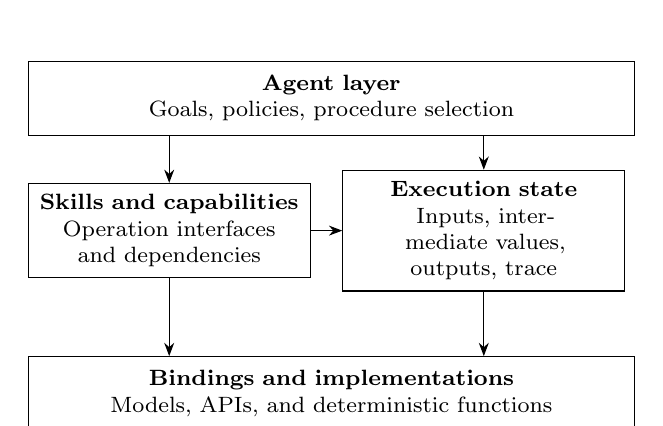
\begin{tikzpicture}[font=\footnotesize,>=Stealth,
box/.style={draw,thin,align=center,inner sep=5pt,text width=7.35cm},
half/.style={draw,thin,align=center,inner sep=4pt,text width=3.30cm}]
\node[box] (agent) {\textbf{Agent layer}\\Goals, policies, procedure selection};
\node[half,below=6mm of agent.south west,anchor=north west] (skill) {\textbf{Skills and capabilities}\\Operation interfaces\\and dependencies};
\node[half,right=4mm of skill] (state) {\textbf{Execution state}\\Inputs, intermediate values,\\outputs, trace};
\node[box,below=28mm of agent] (binding) {\textbf{Bindings and implementations}\\Models, APIs, and deterministic functions};
\draw[->] (agent.south -| skill.north)--(skill.north);
\draw[->] (agent.south -| state.north)--(state.north);
\draw[->] (skill)--(state);
\draw[->] (skill.south)--(binding.north -| skill.south);
\draw[->] (state.south)--(binding.north -| state.south);
\end{tikzpicture}
\caption{The procedural boundary. Skills and capability interfaces describe the task; named state exposes its data; bindings connect the description to execution. The agent retains goal and policy responsibilities.}
\label{fig:model}
\end{figure}

\section{Choosing the Right Procedural Boundaries}

\subsection{Why a Prompt Alone Is an Incomplete Procedure Interface}

Natural-language instructions are flexible. They can express unfamiliar tasks without first constructing a library of typed operations. This makes direct prompting attractive for exploration and for jobs whose process does not need to be reused. The difficulty arises when the same interaction is expected to carry both problem-solving content and the machinery that coordinates its execution.


Chain-of-thought prompting encourages a model to produce intermediate reasoning text \cite{r1}. Such text can be useful, but its presence does not establish a stable interface between operations. It need not provide typed intermediate values, explicit dependency relationships, or executable conditions. Inspecting generated prose and inspecting a declared computation graph are different activities.


Similar concerns arise in loops that interleave reasoning and action \cite{r2} and in systems that enable models to use tools \cite{r3}. Tool access expands what an agent can do. It does not, on its own, define a reusable semantic layer between the task and the tools. If the model also determines control flow inside the interaction, the procedure can remain coupled to the generated output.


The problem is therefore not simply the length of a prompt. It is the absence of independent representations for operation meaning, data movement, and control. A shorter prompt can retain the same coupling, while a multi-call system can still lack consistent interfaces if its steps are assembled ad hoc.


\subsection{When Decomposition Helps}

The appropriate capability boundary is the smallest meaningful unit that provides a practical improvement in reuse, inspection, validation, or control. Meaningful is essential: dividing a task into more steps has no intrinsic value. A unit should correspond to an operation whose inputs, outputs, and role can be understood well enough to make composition useful.


Separating entity extraction from summarization, for example, can expose an intermediate artifact that another workflow might also consume. Separating candidate generation from a later choice can create a point at which criteria or policies are inspected. In both cases, the decomposition is justified by an identifiable boundary, rather than by a desire to maximize the number of calls.


These boundaries can reduce repeated procedural reconstruction. A skill stores an organization that can be invoked again, and a capability provides an interface that other skills can use. This is reuse of structure. It does not mean that a probabilistic capability automatically reuses earlier results or avoids recomputing its own output.


Reuse also changes how systems accumulate functionality. Instead of treating each task as an isolated prompt, a system can develop a library of operations and procedures. The investment in stable interfaces is recovered through repeated use and substitution across tasks. For a one-off task, that investment may not be worthwhile.


\subsection{When Decomposition Hurts}

A tightly coupled operation may have no useful intermediate representation. Splitting it can force the system to expose an unstable artifact that is difficult to validate and that later steps must reinterpret. In such cases, the new boundary can make the procedure more cumbersome without making it more understandable.


Additional boundaries also introduce additional coordination. Inputs must be mapped, implementations resolved, results checked, and state updated. When each step invokes a model, decomposition can add network and inference latency as well as runtime overhead. The total expense must be assessed against the operational benefit of the exposed steps.


PACT therefore discourages decomposition when an operation is already appropriately atomic, when strong semantic coupling makes the interface unreliable, or when orchestration costs exceed gains in inspection and control. A coarse capability remains compatible with the framework if it is the right unit for the task.


Granularity should also be considered across a library. Excessively narrow capabilities can create a fragmented vocabulary with little reuse. Overly broad ones can hide important policy or data boundaries. Designing a capability taxonomy involves a practical judgment about what should stay stable as tasks and implementations change.


\subsection{Human-Defined and Agent-Formed Procedures}

Skills need not be authored exclusively by people. An agent can select a known procedure when one fits its goal, or compose available capabilities into a new procedure when the task is unfamiliar. A useful newly formed composition may subsequently become a reusable skill.


These modes share the same execution representation. The origin of a procedure does not change the need for compatible inputs, valid dependencies, suitable bindings, and applicable policies. Declarative structure provides a common object on which both human review and automated checks can operate.


The broader agent remains responsible for deciding what to attempt, which constraints apply, how to respond to failure, and whether a procedure should be revised. PACT does not claim to solve goal selection or long-term adaptation. It supplies the procedural layer within which a selected course of work can be carried out.


\section{Realizing PACT as an Execution System}

\subsection{From Semantic Objects to Runtime Services}

The composition model requires four cooperating services: a source of capability definitions, a representation of skill definitions, an implementation resolver, and an engine that executes dependencies while maintaining state. These are runtime responsibilities derived from the model, rather than assumptions about a particular deployment technology.


A capability registry preserves the canonical definitions of operation interfaces. Besides input and output descriptions, entries may contain behavioral properties, usage constraints, descriptive metadata, and compatibility information. The registry records what a capability means. Its role is distinct from a catalogue of the particular programs or services currently available to perform it.


The skill-definition layer holds the procedural graphs. It specifies step inputs, output destinations, dependencies, and any relevant branch conditions. Keeping this layer independent of the execution environment allows definitions to be versioned and examined without having to fix every service choice at authoring time.


The resolver associates requested capabilities with implementations. Defaults can provide an ordinary configuration, while environment-specific overrides permit substitution. Selection policies may take account of cost, performance, reliability, or trust. The engine consumes these decisions and carries out the procedure according to its declared relationships.


\subsection{The Reference System and Its Entry Points}

The implementation described in the source manuscript is publicly associated with the pact-research repository at \url{https://github.com/11adyy/pact-research.} It serves here as the concrete realization of the PACT composition model. Its reported design covers a full execution environment, including discovery, scheduling, policy checks, state, and integrations, rather than only a wrapper around model calls.


Developer entry points include a command-line interface for running, describing, scaffolding, and testing skills; an HTTP API with server-sent-event streaming; and SDK integrations. The architecture also includes an MCP server with stdio and SSE transports and native adapters for language-model providers. The interfaces allow different callers to reach a shared skill execution substrate.


The source architecture identifies Python, TypeScript, LangChain, CrewAI, AutoGen, and Semantic Kernel in its SDK and integration surface, and Anthropic, OpenAI, and Gemini in its native model adapter surface. These are reported integration elements of the reference design. They do not alter the capability contract or require each skill to depend directly on the corresponding framework.


A skill gateway sits between these interfaces and the engine. Its responsibilities include discovery, ranking, and governance. This separates the problem of finding an appropriate executable skill from the engine's task of evaluating an already selected procedure.


\begin{figure*}[t]
\centering
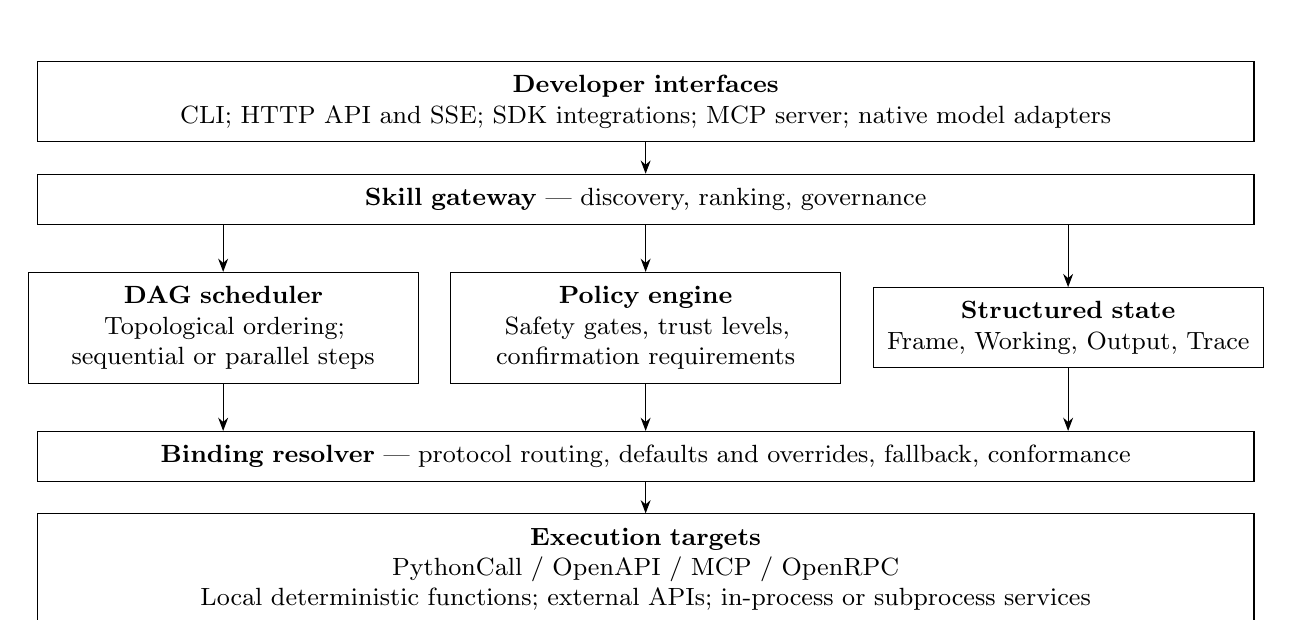
\begin{tikzpicture}[font=\small,>=Stealth,
wide/.style={draw,thin,align=center,inner sep=5pt,text width=15.1cm},
part/.style={draw,thin,align=center,inner sep=5pt,text width=4.6cm}]
\node[wide] (entry) {\textbf{Developer interfaces}\\CLI; HTTP API and SSE; SDK integrations; MCP server; native model adapters};
\node[wide,below=4mm of entry] (gateway) {\textbf{Skill gateway} --- discovery, ranking, governance};
\node[part,below=6mm of gateway] (policy) {\textbf{Policy engine}\\Safety gates, trust levels,\\confirmation requirements};
\node[part,left=4mm of policy] (scheduler) {\textbf{DAG scheduler}\\Topological ordering;\\sequential or parallel steps};
\node[part,right=4mm of policy] (state) {\textbf{Structured state}\\Frame, Working, Output, Trace};
\node[wide,below=6mm of policy] (resolver) {\textbf{Binding resolver} --- protocol routing, defaults and overrides, fallback, conformance};
\node[wide,below=4mm of resolver] (services) {\textbf{Execution targets}\\PythonCall / OpenAPI / MCP / OpenRPC\\Local deterministic functions; external APIs; in-process or subprocess services};
\draw[->] (entry)--(gateway);
\draw[->] (gateway.south -| scheduler.north)--(scheduler.north);
\draw[->] (gateway)--(policy);
\draw[->] (gateway.south -| state.north)--(state.north);
\draw[->] (scheduler.south)--(resolver.north -| scheduler.south);
\draw[->] (policy)--(resolver);
\draw[->] (state.south)--(resolver.north -| state.south);
\draw[->] (resolver)--(services);
\end{tikzpicture}
\caption{Reference runtime organization. The integration surface converges on a gateway and execution substrate, while implementation resolution isolates service-specific transports from procedural definitions.}
\label{fig:runtime}
\end{figure*}

\subsection{Definitions, Names, and Explicit Data Mapping}

The reference system represents capabilities and skills through structured declarative specifications. A skill identifies capability invocations and describes named relationships between their values. Invocation inputs, temporary variables, and final outputs occupy distinct roles in the definition.


This separation prevents the dataflow model from depending on whatever conversational context happens to have accumulated. Each step has a declared source for its parameters and a declared destination for its result. The procedural definition can therefore be examined for missing data or inconsistent relationships before relying on backend behavior to discover an error.


Capability names follow the pattern {\small\urlstyle{tt}\nolinkurl{domain.noun.verb}}. The pattern provides a lightweight taxonomy: related operations can be grouped semantically, and names suggest the kind of entity and operation involved. It helps discovery and reuse without requiring a comprehensive formal ontology.


Behavioral metadata extends this naming layer. Determinism, side effects, and idempotency can inform how execution is governed and how an output should be treated. Naming makes capabilities easier to locate; metadata makes their operational differences explicit. Neither should be mistaken for proof that an implementation satisfies every advertised property.


\subsection{Dependency Scheduling and Constrained Expressions}

The engine derives execution order from declared dependencies. The reference design uses a DAG scheduler with topological ordering and support for sequential and parallel execution. Steps whose prerequisites are satisfied can be scheduled; steps that depend on unavailable results must wait for the corresponding data.


Dependency analysis also provides opportunities to detect missing or incompatible inputs and identify unused or redundant outputs. A workflow graph gives the system something concrete to inspect. A fixed sequence of loosely connected model calls does not necessarily offer the same representation, even when its order is manually obvious.


The implementation includes expressions that read structured state and form step parameters. These expressions support mappings from an earlier result to a later input, conditional parameterization, and lightweight transformations. They are evaluated within a controlled mechanism rather than through unrestricted code execution.


Expression evaluation is consequently part of the declarative interface. It supplies enough flexibility to connect nontrivial intermediate structures while preserving limits on what a workflow expression can execute. Complex computation can remain inside a bound capability, where its interface and implementation are separately identified.


\subsection{The Binding Layer}

The resolver distinguishes ordinary implementations from configuration-specific overrides. A capability can have multiple candidate implementations, with the selected binding determined by context or configuration. This allows development, testing, and production environments to realize the same procedural definition differently.


The reference architecture describes protocol routing, fallback, and conformance responsibilities in this layer. Its execution targets include PythonCall, OpenAPI, MCP, and OpenRPC. The service layer contains local deterministic Python functions, external APIs, and MCP services that can be hosted in-process or reached through subprocesses.


These adapters connect semantic requests to heterogeneous systems. The resolver does not need to collapse those systems into a single kind of computation. A local function and a model-backed service can coexist within one skill because the procedural layer refers to capability interfaces rather than directly encoding each transport.


Substitution is particularly useful for comparing strategies for the same operation. A developer can change a binding and inspect its effect while leaving the surrounding skill intact. This reduces the amount of procedural change needed to investigate differences in cost, latency, or behavior.


\subsection{The Invocation Cycle and State Record}

For each step, the runtime obtains the required inputs from state, resolves a compatible implementation, invokes it, and writes the resulting values to the designated state locations. The scheduler and policy mechanisms determine when and under what conditions this cycle is permitted to proceed.


Each invocation is therefore a separate operational event. Its inputs, outputs, and chosen binding can be recorded, and the system can report progress at step boundaries. This makes it possible to locate an unexpected artifact within the execution path instead of inferring the path only from the final answer.


The reference design identifies its structured state representation as CognitiveState v1, with Frame, Working, Output, and Trace areas. These named areas distinguish execution context, intermediate work, returned artifacts, and execution history. They operationalize the broader distinction between supplied inputs, temporary results, and final outputs.


The trace records executed steps together with their data and bindings. Such a record supports debugging, auditing, and performance analysis. It also creates a basis for future replay, optimization, or verification work, although the existence of a trace alone does not establish that these extensions have already been implemented or validated.


\section{Validation and Accountability at Procedure Boundaries}

\subsection{Observing an Execution}

Once a procedure has explicit steps and addressable state, inspection can refer to particular execution events. A reviewer can ask which capability produced a value, what input it received, and which implementation was selected. The answer can be represented in a structured trace rather than assembled from loosely related prompt logs.


This distinction is operational. A trace exposes the sequence of declared computations and their intermediate artifacts. It need not expose the full internal reasoning of a model-backed implementation, and generated explanations should not be treated as an exhaustive record of that internal computation.


The benefit is nonetheless substantial for system maintenance. A malformed output can be associated with a particular invocation. A missing dependency can be associated with a procedural definition. A backend substitution can be associated with a binding decision. Different failure sources become easier to distinguish because the architecture represents them separately.


\subsection{Enforcing Constraints Before Propagation}

Explicit boundaries create places for checks before one operation's result is consumed by another. At the capability boundary, input and output validation can inspect structure or required conditions. At the skill boundary, declared control and dataflow can constrain the permitted process. At the runtime boundary, execution policies can govern which operations are allowed to proceed.


The reference policy engine is described in terms of safety gates, trust levels, and confirmation requirements. These mechanisms connect governance to execution rather than treating it only as post-processing of a final answer. A result that fails an applicable check can be handled before it becomes an unchecked input to a later operation.


The architectural placement matters more than any particular catalogue of rules. A policy must have a defined point of application and enough information to make its decision. PACT supplies operation identity, interface values, declared properties, and execution context as possible inputs to that decision.


This design supports proactive constraint enforcement. It does not establish that every possible policy is expressible, that every implementation is trustworthy, or that a deployment satisfies a formal safety property. Those conclusions depend on the actual checks, metadata, services, and environment.


\subsection{Trust Depends on the Kind of Operation}

A deterministic transformation, a probabilistic judgment, and an operation with external side effects should not automatically be treated in the same way. Their outputs and repetition behavior have different implications. Explicit capability properties let a workflow or policy make those distinctions at a named boundary.


For a probabilistic capability, additional output validation may be appropriate. For a capability with side effects, policies may restrict invocation or require confirmation. For an idempotent operation, repetition has a different meaning than it has for an operation that changes external state each time. PACT provides a place to describe and act on these differences.


Trust is therefore associated with execution semantics as well as with the identity of a provider. However, a declaration of determinism or idempotency is not itself a verification result. Stronger assurances require evidence about the implementation and the scope under which the property holds.


\subsection{Semantic Checks and Their Limits}

Typed values help detect certain composition errors, but type compatibility is only part of semantic compatibility. A later step may require a result satisfying a precondition that is not captured by the basic shape of the value. A procedure may also rely on an invariant that must remain true across several invocations.


Capability interfaces, skill graphs, and explicit state provide locations for these richer conditions. Preconditions can describe when an operation is applicable; postconditions can describe the expected relationship between input and result; invariants can describe requirements spanning steps. The framework permits such constraints without demanding a fully formalized specification for every skill.


This is a foundation for systematic validation, not a completed formal-verification method. Structured execution can make failures visible and checks enforceable while still depending on uncertain model outputs. Governance benefits from the representation, but it also requires substantive policies and valid implementations.


\section{Relationship to Other Agent Design Approaches}

PACT addresses an abstraction boundary that intersects several strands of agent research. Chain-of-thought methods organize generated reasoning text \cite{r1}. ReAct couples reasoning with actions in an interaction pattern \cite{r2}. Toolformer studies language-model tool use \cite{r3}. MRKL Systems develops a modular arrangement of models, knowledge sources, and discrete reasoning \cite{r4}. These approaches motivate different aspects of structured behavior, but they do not all make the same commitments about semantic interfaces, declarative procedure definitions, or runtime-managed state.


Graph of Thoughts and least-to-most prompting provide further perspectives on organizing reasoning work [5, 6]. Their relevance is the value of structure beyond an undifferentiated prompt. PACT focuses on an execution representation through which such operations can be composed, bound to services, inspected, and governed.


Frameworks such as LangChain offer integrations and orchestration facilities \cite{r7}, while AutoGen emphasizes multi-agent conversation \cite{r8}. PACT can coexist with these facilities. Its reference design includes framework-facing integration points precisely because a procedural runtime can sit beneath or alongside an agent's broader orchestration layer.


The important comparison is architectural rather than a ranking of complete products. A framework's users may implement declarative workflows, binding layers, state, or tracing even if those features are not central to a simple usage pattern. Conversely, having a workflow API does not automatically establish stable semantic contracts across all operations.


\begin{table*}[t]
\centering
\caption{Qualitative comparison of representative architectural patterns, retained from the source account. Entries describe patterns rather than exhaustive framework capabilities.}
\label{tab:comparison}
\small
\begin{tabular}{@{}p{7cm}lll@{}}
\toprule
Architectural concern & PACT & LangChain-style & ReAct-style\\
\midrule
Declarative procedures & Explicit & Partial & Absent\\
Late implementation binding & Explicit & Partial & Absent\\
Structured execution state & Explicit & Limited & Absent\\
Reusable capability units & Explicit & Partial & Absent\\
Step-level observability & Explicit & Partial & Limited\\
\bottomrule
\end{tabular}
\end{table*}

Table 1 summarizes the contrast made in the source manuscript between the proposed design, a LangChain-style orchestration pattern, and a ReAct-style interaction loop. The qualitative entries refer to those representative patterns, not to every version, extension, or possible configuration of the named frameworks. They identify which concerns PACT treats as first-class objects.


The distinctive commitment is that operation meaning, procedural organization, implementation choice, and execution state are separately represented. This commitment makes reusable capabilities and runtime-level validation direct architectural concerns. It does not require abandoning prompting, tools, or conversational orchestration; those mechanisms can remain inside bound operations or in the agent layer.


\section{Evaluation: Original Benchmark and Extended Systems Study}

\subsection{Question and Comparison}

The evaluation asks how execution organization changes operational behavior when model choice is held constant. It compares a direct strategy that handles an entire task in one model invocation with a structured strategy that invokes capabilities through a declarative skill. The numerical results below are retained from the source evaluation; no additional benchmark run is claimed in this manuscript.


The comparison is aimed at latency, component reuse, visibility of intermediate artifacts, output variation, and structural usability. It is not a test of whether the proposed architecture achieves state-of-the-art reasoning quality. This focus is important because the main argument for PACT concerns how a system executes and exposes its work.


The direct baseline minimizes the number of model calls by placing the full task in a prompt. The structured configuration distributes the task across explicit invocations. Differences in the observed executions therefore include the effects of multi-call decomposition as well as runtime coordination; the measurements do not isolate a pure scheduling overhead.


\subsection{Tasks and Procedural Definitions}

The first task is constrained decision-making: selecting an option from alternatives under stated evaluation criteria. The structured skill is {\small\urlstyle{tt}\nolinkurl{experiment.structured-decision.}} Its capability sequence requests candidate generation through {\small\urlstyle{tt}\nolinkurl{agent.option.generate}} and then uses {\small\urlstyle{tt}\nolinkurl{agent.flow.branch}} for the selection-related stage.


The second task is a text-processing composition with entity extraction, summarization, and classification. Its skill is {\small\urlstyle{tt}\nolinkurl{experiment.text-processing-pipeline}}, using {\small\urlstyle{tt}\nolinkurl{text.entity.extract}}, {\small\urlstyle{tt}\nolinkurl{text.content.summarize}}, and {\small\urlstyle{tt}\nolinkurl{text.content.classify}} in sequence. The task exposes intermediate artifacts that a single-call baseline can otherwise leave inside one interaction.


Both task families were executed with 10 inputs per task and both strategies. Output variability was examined on 3 inputs with 3 repetitions per input. The reported runs used GPT-4o-mini and a fixed random seed of 42. They were carried out locally on a laptop, without distributed infrastructure.


Holding the model constant narrows the comparison to the evaluated execution configurations. It does not make the runs deterministic, nor does it remove the influence of prompt differences and multiple invocations. The small task set also limits how far the observations can be generalized.


\subsection{What Was Measured}

Latency is the total wall-clock duration of a task execution. Traceability records whether intermediate steps are externally observable. Reusability records whether an operation is available as an independently composable component. The latter two dimensions are chiefly properties of the evaluated system organization rather than task-quality scores.


Variability is represented by Jaccard distance across repeated outputs for identical inputs. The reported result provides a descriptive indication of output differences in this setup. It does not establish a distribution-wide stability guarantee or identify which particular step contributed most to the variation.


Output validity is a qualitative assessment of whether the returned artifacts are structurally usable. The evaluation does not measure semantic correctness or optimality against external ground truth, and it does not include a human accuracy assessment. A structurally valid answer can still be wrong; these categories must therefore remain distinct.


\subsection{Observations}

\begin{table*}[t]
\centering
\caption{Operational observations from the source evaluation. Variability is reported as Jaccard distance; validity is qualitative. Neither measures semantic accuracy.}
\label{tab:results}
\small
\begin{tabular}{@{}p{7.4cm}ll@{}}
\toprule
Reported dimension & Single-call prompt & Structured procedure\\
\midrule
Mean decision latency & 4.79 s & 12.17 s\\
Mean text-processing latency & 2.93 s & 7.86 s\\
Intermediate execution trace & Not exposed & Step-level\\
Independent component reuse & Not exposed & Capability-level\\
Text-output variability & $\sim$0.12 & $\sim$0.17\\
Qualitative output validity & High & High\\
\bottomrule
\end{tabular}
\end{table*}

The direct strategy was faster on both task families. Mean decision-task latency was 4.79 seconds for the single-call baseline and 12.17 seconds for structured execution. For text processing, the corresponding means were 2.93 and 7.86 seconds. The ratios are approximately 2.54 and 2.68, respectively.


The structured configuration supplied step-level traces and separately reusable capability interfaces. The single-call baseline did not expose equivalent intermediate execution steps or capability-level components in the tested arrangement. These observations match the representational distinction between a prompt that requests a whole result and a procedure whose invocations are independently identified.


Both strategies received a high qualitative output-validity assessment. This supports the limited observation that decomposition did not prevent production of usable output structures in the tested tasks. It does not demonstrate equal semantic quality, superior accuracy, or reliable performance outside the evaluated examples.


Reported text-processing variability increased from approximately 0.12 in the baseline to approximately 0.17 in the structured configuration. Multi-step generation may accumulate differences across stages, which is consistent with this observation. The evaluation does not supply enough evidence to establish that mechanism as the sole cause or to infer a general variability penalty for all structured workflows.


\subsection{What the Comparison Supports}

In the original benchmark, the strongest empirical result is the added elapsed time in these two configurations. A procedure containing several model-backed steps takes longer than a baseline that requests a complete answer in one call. Its justification must therefore come from the value of its boundaries, not from a claim that decomposition automatically accelerates the task.


The inspection and reuse benefits are visible in the system design and demonstrated by the availability of named steps and components. The original measurements do not quantify long-term engineering savings from reuse, reduced debugging time, or governance effectiveness. The extended study below adds mechanical substitution and policy probes, while leaving human maintenance benefits unmeasured.


The comparison also warns against equating structure with stability. Explicit steps identify where variability can occur, but they can add probabilistic stages. Better localization of uncertainty and lower aggregate variation are different goals, and the evaluated configuration does not achieve both by construction.


\subsection{Extended Evaluation: Evidence and Protocol}

The initial benchmark motivates a more direct test of the runtime's architectural claims. We extend it with a controlled systems study that separates execution correctness, governance, implementation substitution, and orchestration cost from language-model quality. The supplied runtime is evaluated without modifying its source. Actual YAML definitions pass through the native loaders, planner, engine, scheduler, state mappings, binding resolver, and PythonCallInvoker. Controlled Python services replace model inference so that task answers and injected faults are known in advance.


The evidence has three distinct origins. Sections 7.1--7.5 retain the benchmark reported in the original manuscript; those historical model calls were not rerun for this extension. Sections 7.6--7.11 report newly executed offline trials with raw records. Section 7.12 records additional author-reported LLM aggregates, which have no accompanying trial logs and remain unverified. Neither the historical observations nor the reported LLM aggregates enter the new trial count.


Four generated task families cover integer summation, maximum selection, constrained weighted choice, and tagged-text extraction followed by aggregation. An independent exact oracle computes the expected value and label. Oracle-only fields are removed from service inputs. Decision instances contain eligible and ineligible alternatives, criteria weights, and an explicit tie rule; text instances include tagged values and irrelevant text. These are controlled system workloads, not a benchmark of open-ended agent reasoning.


The healthy protocol contains 100 distinct inputs per family, three repetitions per input, and eight execution arms: 9,600 recorded runs. Fault and policy experiments contain 16 scenarios, each applied to 100 distinct inputs across the eight arms: 12,800 runs. Additional probes contribute 30 structural-invalidity runs, 160 before/after substitution executions, 600 chain-scaling runs, and 192 fan-out runs. The total is 23,382 executions; deterministic repetitions are not counted as additional independent task cases.


The random seed is 20261002. Healthy and chain jobs use seeded randomized order, with an excluded warmup for each arm. Real wall-clock elapsed time is measured with {\small\urlstyle{tt}\nolinkurl{perf_counter_ns}}. Setup is outside per-trial timing, logging is suppressed, and audit persistence is disabled. Each trial resets the circuit breaker; slow-fault trials include a separate observation wait to capture late effects before the next trial starts. Effects are confined to an in-memory ledger, with no production writes.


\subsection{Matched Baselines and Statistical Units}

\begin{table*}[t]
\centering
\caption{Extended-study execution arms. The primary comparator matches five service invocations and declared governance checks; the direct and transport arms are supplemental lower bounds.}
\label{tab:arms}
\small
\setlength{\tabcolsep}{4pt}
\renewcommand{\arraystretch}{1.12}
\begin{tabularx}{\textwidth}{@{}p{3.3cm}X@{}}
\toprule
Arm & Execution configuration\\
\midrule
direct & Shared workload functions called directly\\
transport & Same functions through the native PythonCallInvoker and per-call threads\\
manual\_guarded & Transport plus independent type/policy checks and the same integrity gate\\
pact & Full native runtime, contracts, scheduling, state mapping, binding resolution, and gates\\
pact\_no\_policy & Loader adapter removes safety metadata; runtime source unchanged\\
pact\_no\_validation & Bypass capability validation/enrichment; planning, response mapping and transport retained\\
pact\_trace\_off & Public trace\_enabled=False; actual structured trace contents recorded\\
pact\_static\_binding & Freeze initial native resolver choices; remaining layers retained\\
\bottomrule
\end{tabularx}
\end{table*}
The primary cost comparison is full PACT against {\small\urlstyle{tt}\nolinkurl{manual_guarded}}. Both invoke four workload operations (normalization, solving, verification, and commit) plus the same post-solver integrity gate. The scripted comparator implements independent trust, confirmation, tenant, and input/output checks over the same invoker. Its output-type validation is stricter than the current native implementation. The comparison therefore matches computation and the declared governance workload, while retaining differences in how the checks are implemented.


The direct and transport arms omit the integrity gate and are supplemental lower bounds. They cannot isolate the overhead of governance-equivalent execution. Likewise, the validation ablation retains response mapping, planning, and transport; it does not remove every check. The trace ablation uses the public {\small\urlstyle{tt}\nolinkurl{trace_enabled=False}} option rather than assuming complete suppression of trace construction.


Healthy correctness requires completion and exact equality of the returned value and label with the oracle. A case-level success requires every repetition of that input to succeed. Mean-latency intervals use 2,000 seeded bootstrap resamples of per-case average latency; primary latency differences are paired on the same case. Wilson intervals describe case-level success coverage. These intervals concern the generated test inputs and do not estimate a deployment-wide safety probability.


\subsection{Healthy Execution and Orchestration Cost}

\begin{table*}[t]
\centering
\caption{Healthy deterministic workloads: 100 distinct inputs per family, three repetitions. Success requires exact oracle agreement in every repetition. Latency is in milliseconds; the paired-difference interval uses case bootstrap resampling.}
\label{tab:healthy-extended}
\small
\setlength{\tabcolsep}{4pt}
\renewcommand{\arraystretch}{1.12}
\begin{tabularx}{\textwidth}{@{}Xlllll@{}}
\toprule
Task & PACT cases & PACT mean & Manual mean & Paired delta & 95\% interval\\
\midrule
sum & 100/100 & 12.081 & 0.586 & 11.494 & [11.366, 11.673]\\
max & 100/100 & 12.096 & 0.601 & 11.495 & [11.387, 11.609]\\
decision & 100/100 & 12.139 & 0.729 & 11.411 & [11.334, 11.486]\\
text & 100/100 & 12.250 & 0.611 & 11.639 & [11.387, 12.065]\\
\bottomrule
\end{tabularx}
\end{table*}
Full PACT returns the exact expected answer in 1,200 of 1,200 healthy runs, comprising 400 distinct inputs. Each family has 100 of 100 cases correct in all three repetitions. The corresponding family-level Wilson 95\% interval is approximately [0.963, 1.000]. All other healthy arms also achieve exact outputs on all 1,200 runs per arm. This result shows preservation of the controlled computations; it provides no evidence that PACT improves their task-solving accuracy.


PACT's mean latency ranges from 12.081 to 12.250 ms across the four families. Relative to the manually guarded comparator, paired mean differences range from 11.411 to 11.639 ms. Table 4 reports case-bootstrap intervals for those differences. This is measured local coordination cost over deterministic services, not a model-inference latency or an estimate of model-call savings.


The measured scope includes YAML loading during execution, planning, scheduling, mapping, binding invocation, checks, and instrumentation in a warm process. Cold component construction is recorded as one observation per arm, without a confidence interval. The environment reports Python 3.12.14 and 9 reported CPUs; it is a shared Linux host with no CPU pinning or control over other tenants. A regression-check process briefly overlaps the beginning of the healthy run. Randomization reduces systematic ordering bias, but the timing intervals remain descriptive of this session and are not hardware-independent guarantees.


\subsection{Faults, Policies, and Effects After Failure}

\begin{table*}[t]
\centering
\caption{Expected-behavior counts on 100 distinct inputs per scenario. Recovery requires exact output; containment requires failure without an effect. Terminal output is scored for rejection. The transport arm has no policy or deadline guard.}
\label{tab:faults-extended}
\small
\setlength{\tabcolsep}{4pt}
\renewcommand{\arraystretch}{1.12}
\begin{tabularx}{\textwidth}{@{}Xlll@{}}
\toprule
Scenario & Transport & Manual guarded & PACT\\
\midrule
service exception & 100/100 & 100/100 & 100/100\\
missing output & 100/100 & 100/100 & 100/100\\
wrong intermediate type & 0/100 & 100/100 & 100/100\\
null intermediate & 0/100 & 100/100 & 0/100\\
negative semantic result & 0/100 & 100/100 & 100/100\\
plausible wrong result & 0/100 & 0/100 & 0/100\\
terminal output type & 0/100 & 100/100 & 0/100\\
low trust & 0/100 & 100/100 & 100/100\\
unconfirmed effect & 0/100 & 100/100 & 100/100\\
cross tenant & 0/100 & 100/100 & 100/100\\
missing tenant & 0/100 & 100/100 & 100/100\\
missing target tenant & 0/100 & 100/100 & 0/100\\
transient recovered & 100/100 & 100/100 & 100/100\\
transient no retry & 100/100 & 100/100 & 100/100\\
step timeout & 0/100 & 100/100 & 100/100\\
late effect after timeout & 0/100 & 0/100 & 0/100\\
\bottomrule
\end{tabularx}
\end{table*}
Each scenario declares an expected outcome before execution. Containment requires failed execution and no ledger effect; recovery requires an exact oracle result; a terminal-output probe requires rejection and is not credited with containment merely because an error could be detected after a write. Raw records retain detection, completion, correctness, calls, downstream activity, failure-step identifiers, binding choices, and effects separately. A zero or full success count over 100 cases has a Wilson 95\% interval of approximately [0.000, 0.037] or [0.963, 1.000], respectively.


PACT blocks all 100 requests in each low-trust, unconfirmed, explicit cross-tenant, and missing-caller-tenant scenario before the commit effect. Exceptions, missing output fields, intermediate type mismatches, and a negative result forbidden by the declared invariant are also contained in all tested cases. With configured retries, the deliberately transient solver failure recovers to the correct result in 100 of 100 cases; without retries, it stops before commit. These outcomes concern specified fixtures, not arbitrary adversarial tools.


Five probes expose limitations in the present implementation. A null intermediate output is accepted and execution completes with an unusable final result in every tested case; the controlled commit service records no effect for this null value, but the runtime does not reject it. A plausible positive wrong answer passes the nonnegative-value gate and reaches commit in all 100 cases. A terminal output with an invalid type also completes in all 100 cases, after the effect has occurred. Missing target-tenant information is accepted in all 100 cases despite the intended same-tenant requirement. These observations distinguish required-field checks and simple invariants from complete type and semantic validation.


The timeout experiments distinguish detection from stopping the underlying work. A delayed solver times out and prevents downstream commit in all 100 cases. A delayed commit, however, writes its ledger effect after the timeout in all 100 cases. The engine reports failure, but the Python worker is not cancelled in a way that prevents completion. A deadline notification therefore does not establish effect containment; stronger cancellation, transactional boundaries, or operation-specific compensation is needed for consequential actions.


Unknown dependencies, cyclic graphs, and writes to read-only state are rejected before any service call in all 30 structural probes. This verifies those three malformed definitions only, rather than proving every scheduling and state invariant.


\subsection{Ablations, Trace Behavior, and Reuse}

\begin{table*}[t]
\centering
\caption{Selected ablation outcomes: expected behavior over 100 inputs. Other checks remain active when capability validation is bypassed; failure at a retained layer can therefore mask the ablated check.}
\label{tab:ablations-extended}
\small
\setlength{\tabcolsep}{4pt}
\renewcommand{\arraystretch}{1.12}
\begin{tabularx}{\textwidth}{@{}Xlll@{}}
\toprule
Scenario & Full PACT & No safety metadata & No capability validation\\
\midrule
low trust & 100/100 & 0/100 & 100/100\\
unconfirmed effect & 100/100 & 0/100 & 100/100\\
cross tenant & 100/100 & 0/100 & 100/100\\
missing output & 100/100 & 100/100 & 100/100\\
wrong intermediate type & 100/100 & 100/100 & 0/100\\
negative semantic result & 100/100 & 0/100 & 100/100\\
\bottomrule
\end{tabularx}
\end{table*}
Removing safety metadata eliminates the observed trust, confirmation, and cross-tenant blocks, and disables the mandatory invariant gate. Bypassing capability validation allows the intermediate-type mismatch to propagate, while missing outputs can still be rejected by retained response mapping. An unchanged result under this ablation is therefore not proof that capability validation has no function: other layers remain active.


The trace-off arm still contains four structured step records on every healthy execution. It does not implement an experimentally demonstrated removal of all tracing work, so its timing cannot be interpreted as the cost of a trace-free runtime. Traces do expose step identifiers, state lineage, and binding selections. No human debugging-time experiment was performed.


Four workflows reuse four workload capability interfaces. A substitution probe switches the solver to a distinct compatible implementation using one active-map override and no changes to skill files. Each of 40 before/after pairs resets the active selection before testing the swap. Native resolution follows the alternate binding in 40 of 40 pairs and preserves exact output. A frozen-binding ablation follows it in zero of 40 pairs, while remaining correct with the original implementation. This measures compatibility and edit footprint; it does not quantify human productivity or validate arbitrary interchangeable services.


\subsection{Scaling and Independent Branches}

\begin{table*}[t]
\centering
\caption{Matched identity-chain microbenchmarks, 20 runs per length/delay/arm. All time columns are milliseconds; delays are artificial service delays. Paired differences compare native PACT with transport.}
\label{tab:scaling-extended}
\small
\setlength{\tabcolsep}{4pt}
\renewcommand{\arraystretch}{1.12}
\begin{tabularx}{\textwidth}{@{}Xlllll@{}}
\toprule
Steps & Delay/call & Transport mean & PACT mean & Paired delta & 95\% interval\\
\midrule
1 & 0 & 0.16 & 3.39 & 3.22 & [3.12, 3.33]\\
2 & 0 & 0.29 & 5.54 & 5.24 & [5.10, 5.41]\\
8 & 0 & 0.87 & 18.40 & 17.53 & [17.19, 17.86]\\
16 & 0 & 1.63 & 34.09 & 32.47 & [31.79, 33.19]\\
32 & 0 & 2.82 & 68.26 & 65.45 & [64.46, 66.53]\\
1 & 1 & 1.26 & 4.57 & 3.31 & [3.17, 3.46]\\
2 & 1 & 2.49 & 7.80 & 5.31 & [5.15, 5.47]\\
8 & 1 & 9.83 & 27.16 & 17.33 & [17.03, 17.64]\\
16 & 1 & 19.67 & 54.38 & 34.71 & [32.83, 37.71]\\
32 & 1 & 39.39 & 103.78 & 64.39 & [62.91, 66.02]\\
\bottomrule
\end{tabularx}
\end{table*}
Matched identity chains have lengths 1, 2, 8, 16, and 32, with declared service delays of either zero or 1 ms per call. There are 20 runs per length/delay/arm for transport, native PACT, and frozen bindings, giving 600 executions. Table 7 presents mean durations and paired native-minus-transport differences. The added elapsed time increases with chain length in the tested configuration. Artificial service delays remain labeled and are not treated as inference timings.


\begin{table*}[t]
\centering
\caption{Independent branches plus merge, 5 ms branch delay, 12 runs per configuration. Mean elapsed time is in milliseconds. Completion and declared call count succeed for both arms in every configuration.}
\label{tab:fanout-extended}
\small
\setlength{\tabcolsep}{4pt}
\renewcommand{\arraystretch}{1.12}
\begin{tabularx}{\textwidth}{@{}Xllllp{3.1cm}@{}}
\toprule
Branches & Transport, 1 worker & Transport, 4 workers & PACT, 1 worker & PACT, 4 workers & PACT success\\
\midrule
1 & 5.63 & 5.63 & 14.79 & 11.03 & 12/12 at both settings\\
2 & 10.94 & 5.78 & 18.23 & 13.36 & 12/12 at both settings\\
4 & 21.39 & 6.36 & 33.01 & 18.10 & 12/12 at both settings\\
8 & 42.79 & 11.96 & 63.39 & 32.02 & 12/12 at both settings\\
\bottomrule
\end{tabularx}
\end{table*}
Fan-out tests use one, two, four, or eight independent branches followed by a merge, with one or four workers and a controlled 5 ms branch delay. Each configuration has 12 runs under PACT and matched scripted thread-pool transport, yielding 192 executions. All runs complete with exactly the declared branch-plus-merge call count. More workers reduce elapsed time for wider graphs in this workload, subject to orchestration and thread overhead. These results cover independent branches and a merge, not concurrent users, distributed execution, resource saturation, or asynchronous cancellation.


\subsection{Additional Author-Reported LLM Aggregates}

\begin{table*}[t]
\centering
\caption{Additional author-reported LLM aggregates (unverified). No original trial records accompany these values; they are not included in the independently measured execution count.}
\label{tab:llm-reported}
\small
\setlength{\tabcolsep}{4pt}
\renewcommand{\arraystretch}{1.12}
\begin{tabularx}{\textwidth}{@{}Xlll@{}}
\toprule
Reported metric & Single call & Manual, 3 calls & PACT, 3 calls\\
\midrule
Exact-output rate & 86\% & 92\% & 92\%\\
Inputs correct in all three repetitions & 78/100 & 87/100 & 88/100\\
Mean elapsed time & 1.80 s & 4.90 s & 4.92 s\\
Mean total tokens per execution & 678 & 1,378 & 1,378\\
\bottomrule
\end{tabularx}
\end{table*}
The author additionally reports the aggregates in Table 9, adopting a design of 100 distinct inputs and three repetitions. These values coincide with an earlier hypothetical illustration except for the reported token totals of 678 and 1,378. No original outputs, provider usage records, timestamps, model identifier, or matched trial files accompany them. They are retained as author-reported, unverified aggregates, rather than added to the independently measured evidence or treated as an executed experiment in this environment. Confidence intervals and significance claims cannot be recovered from the supplied aggregates alone.


Conditionally, if the underlying records substantiate the table, staged execution improves exact-answer rate by six percentage points relative to the single-call configuration. The manual and PACT staged configurations have equal reported accuracy and token totals. PACT's reported mean latency is 20 ms higher than the staged manual comparator; the one-input difference in all-repeat success is insufficient evidence of an accuracy advantage. Staged execution uses about 2.03 times the reported tokens of the single-call configuration, rather than demonstrating a token saving.


The implemented opt-in live runner is available for a verified comparison. It uses the same staged prompts, parsing, functions, model settings, and exact oracles across transport, manually guarded execution, and PACT; it also includes a single-call comparator, per-trial usage and errors, randomized order, and an API-call cap. It performs no deterministic fallback. No API credentials were present during the measured offline study, so no model requests were executed for that study. The supplied aggregate table has no unguarded staged-transport row; that result is not inferred.


\subsection{Reproducibility and Scope of the Evidence}

The experiment package contains generated YAML fixtures, the seeded dataset, scenario definitions, raw JSONL/JSON, summaries, source hashes, and reproduction commands. Integrity checks verify 78 runtime and eight evaluation Python source hashes, dataset and fixture hashes, the 23,382-execution denominator, unique healthy trial keys, and agreement between stored correctness flags and oracle comparisons. The measured runtime source is unchanged. The harness has 29 passing tests and passes its lint checks.


A relevant existing runtime test subset has 65 passing tests and one failure: {\small\urlstyle{tt}\nolinkurl{test_local_selection_keeps_terminal_official_default_safety_net}} expects an official OpenAPI fallback in a locally selected Python binding chain, but that fallback is absent. This failure predates the experiment harness and is preserved in the validation log. Results should not be interpreted as a fully passing runtime regression suite.


The new study supports bounded claims about correct execution of these deterministic workflows, specified policy checks, compatible implementation substitution, and measured coordination cost. It exposes concrete validation and timeout-effect weaknesses. It does not establish better LLM reasoning, prompt-injection resistance, real-world generalization, developer-time savings, provider-independent performance, or safety of arbitrary tools. Audit persistence, production effects, and distributed deployments remain outside the measured scope.


\FloatBarrier

\section{Deployment Trade-offs and Remaining Work}

\subsection{Paying for Boundaries}

Procedural structure incurs two kinds of investment. At design time, developers define capability interfaces, organize skills, and maintain metadata and bindings. At execution time, the system resolves implementations, moves state, performs checks, and may issue multiple model or service calls. Neither expense should be hidden behind a general claim of architectural elegance.


The return depends on how the system is used. A task that is performed once, requires little inspection, and has no important intermediate constraints may be best served by direct prompting. A recurring process with shared operations, policy-sensitive steps, or difficult debugging requirements provides more opportunities for the investment to pay off.


Structured execution offers control points at which an intermediate result can be inspected, a backend replaced, or a policy enforced. Those points have a concrete operational value, but their value is application-dependent. The reported latency increase is therefore a cost to weigh against specific requirements rather than a universal acceptable overhead.


\subsection{Flexibility, Portability, and Semantic Consistency}

Direct natural-language prompting accommodates arbitrary requests with relatively little preparation. A capability library introduces a vocabulary that must be designed and maintained. Users of the library must express work through its available interfaces or create additional ones. This initial friction is the counterpart of stable, reusable composition.


PACT moves part of the flexibility into the construction of procedures and the selection of implementations. The same skill can be bound to different services, and the same capability can participate in different skills. An agent can also form a new composition instead of being restricted to a fixed list of procedures.


These freedoms depend on semantic consistency. If similarly named capabilities have incompatible meanings, or if a replacement backend satisfies the output schema while changing the operation's intended meaning, composition becomes fragile. Managing a growing library therefore requires attention to contracts, compatibility, and capability granularity.


Portability also carries behavioral differences. A backend selected for cost can differ from one selected for reliability; a local deterministic implementation can differ from a probabilistic model call. Explicit bindings make such choices visible, but do not eliminate the need to evaluate them.


\subsection{Appropriate Operational Settings}

PACT is most relevant where a process must be accountable as well as productive. Enterprise operations, regulated workflows, and settings with consequential side effects can benefit from known interfaces, inspectable state, validation gates, and explicit policy decisions. The representation makes these concerns part of the execution substrate.


Such settings also demand more than a representation. A trace does not prove that a decision was correct. A typed interface does not prove that a service obeyed its semantic contract. A policy hook does not establish that the deployed policy is sufficient. The framework makes these obligations easier to place and investigate while leaving their substantive fulfillment to the system design.


In exploratory or low-stakes work, fewer requirements may justify fewer boundaries. PACT can coexist with direct prompting in a broader agent: a model can handle a loosely specified exploratory request, while a reusable procedure handles a task whose sequence and constraints have become established.


\subsection{Limitations of the Present Evidence}

The original model benchmark covers two task families, a small input set, one model, and a local environment; its historical calls were not rerun. The extended systems study adds four deterministic families, paired comparisons, uncertainty intervals, fault injection, and local graph-scaling probes. Its synthetic cases do not establish performance on held-out operational tasks or distributed services. Shared-host timings and disabled audit persistence further limit cost generalization. The additional LLM aggregates lack original trial records and are not independently validated.


The architectural comparison likewise concerns representative design styles. It should not be read as a comprehensive survey showing that other frameworks cannot provide state, tracing, late binding, or reusable workflows. PACT's claim is that these concerns are organized around explicit semantic capabilities and procedural artifacts.


Finally, the runtime cannot remove uncertainty from probabilistic components simply by scheduling them explicitly. Decomposition may improve inspection while increasing elapsed time and output variation. Governance mechanisms can constrain the execution process while still depending on imperfect validators and capability implementations.


\subsection{Directions for Further Development}

The observed validation gaps and effects after timeout make stricter output contracts, fail-closed target checks, and effect-safe cancellation or compensation immediate implementation priorities. Fixes should be evaluated in a new before/after run while retaining the current evidence. Reducing coordination and multi-call latency is also a practical priority for time-sensitive deployments. The structured representation provides information with which execution strategies can be examined, but any optimization must preserve the boundaries that motivated the design. The current results do not establish an optimized runtime configuration.


Another direction is the generation and refinement of skills from available capabilities. New procedures need checks for interface compatibility, useful granularity, and policy adherence before reuse. How to maintain a coherent library as these procedures accumulate remains an open engineering question.


Richer behavioral constraints could strengthen validation, while more detailed trace analysis could help identify where variation and failures arise. Further work may also investigate how adaptive or learning mechanisms interact with explicit procedures. These are prospective extensions, rather than requirements of the current composition model or demonstrated outcomes of the reported benchmark.


\balance\thispagestyle{fancy}

\section{Conclusion}

PACT gives agent behavior a procedural representation whose parts can be examined and changed independently. A skill organizes the task; capabilities name its operations; state carries its information; and bindings connect the semantic requests to executable mechanisms. The runtime follows from these commitments, providing dependency scheduling, state access, service resolution, tracing, and policy application.


This organization supports reuse and inspection at identifiable boundaries. The original model benchmark reports greater latency and slightly greater text-output variation under structured execution. The extended controlled study preserves exact outputs, demonstrates compatible implementation substitution without editing skills, and verifies selected policy and fault paths, with measurable local orchestration cost. It also shows that some invalid outputs and missing target context are accepted, and that timeout detection does not prevent every subsequent effect. These findings establish both tested behavior and current implementation limits.


The resulting case for PACT is conditional and practical. Where procedural knowledge is worth preserving, intermediate results need inspection, and execution must obey explicit constraints, a runtime for reusable skills provides a useful systems abstraction. Its purpose is to make those processes manageable while retaining the expressive capabilities of the models and services that implement them.


\begin{thebibliography}{8}
\small

\bibitem{r1} Jason Wei, Xuezhi Wang, Dale Schuurmans, Maarten Bosma, Brian Ichter, Fei Xia, Ed Chi, Quoc V. Le, and Denny Zhou. Chain-of-thought prompting elicits reasoning in large language models. arXiv:2201.11903, 2022.

\bibitem{r2} Shunyu Yao, Jeffrey Zhao, Dian Yu, Nan Du, Izhak Shafran, Karthik Narasimhan, and Yuan Cao. ReAct: Synergizing reasoning and acting in language models. arXiv:2210.03629, 2023.

\bibitem{r3} Timo Schick, Jane Dwivedi-Yu, Roberto Dessi, Roberta Raileanu, Maria Lomeli, Eric Hambro, Luke Zettlemoyer, Nicola Cancedda, and Thomas Scialom. Toolformer: Language models can teach themselves to use tools. arXiv:2302.04761, 2023.

\bibitem{r4} AI21 Labs. MRKL Systems: A modular, neuro-symbolic architecture that combines large language models, external knowledge sources and discrete reasoning. Technical report, 2022.

\bibitem{r5} Maciej Besta, Nils Blach, Lukas Gianinazzi, Joanna Gajda, Jan Kubicek, Robert Gerstenberger, Mariusz Nyczyk, and Torsten Hoefler. Graph of Thoughts: Solving elaborate problems with large language models. arXiv:2308.09687, 2023.

\bibitem{r6} Denny Zhou, Nathanael Scharli, Le Hou, Jason Wei, Nathan Scales, Xuezhi Wang, Dale Schuurmans, Claire Cui, Olivier Bousquet, Quoc V. Le, and Ed Chi. Least-to-most prompting enables complex reasoning in large language models. arXiv:2205.10625, 2022.

\bibitem{r7} LangChain. LangChain. \url{https://www.langchain.com,} 2023.

\bibitem{r8} Qingyun Wu, Gagan Bansal, Jieyu Zhang, Yiran Wu, Beibin Li, Erkang Zhu, Li Jiang, Xiaoyun Zhang, Chi Wang, et al. AutoGen: Enabling next-gen LLM applications via multi-agent conversation. arXiv:2308.08155, 2023.

\end{thebibliography}
\end{document}